

\begin{frame}[ctb!]
  \frametitle{Nested Components}
  \begin{figure}[h!]
    \begin{center}
      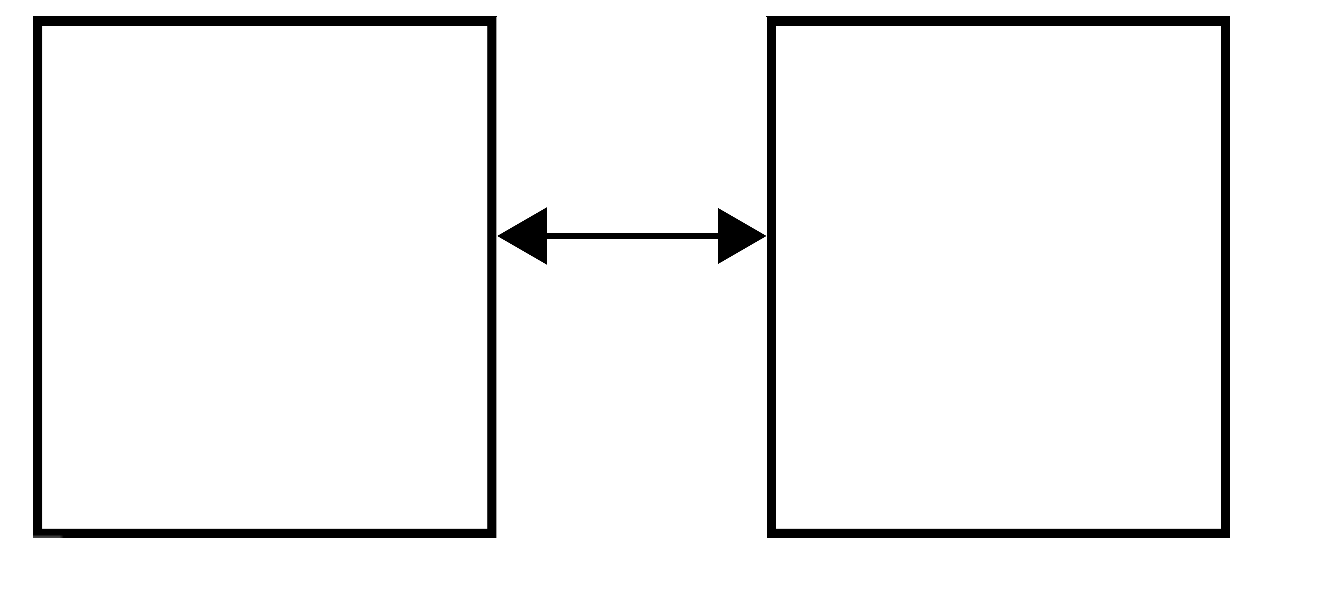
\includegraphics[width=\textwidth]{../report/chapters/paradigm/flow.eps}
    \end{center}
    \caption{The nested components supply thermal flux and concentration 
    information to each other at the boundaries.}
    \label{fig:flow}
  \end{figure}
\end{frame}

\begin{frame}[ctb!]
  \frametitle{Waste Stream}
  % Waste Stream
  A material may be any arbitrary isotopic vector
\end{frame}

\begin{frame}[ctb!]
  \frametitle{Waste Form}
  % Waste Form
  \begin{figure}[h!]
    \begin{center}
      \includegraphics[height=.6\textwidth]{../report/chapters/future/contaminated.eps}
    \end{center}
  \end{figure}
\end{frame}

\begin{frame}[ctb!]
  \frametitle{Waste Form}
  % Waste Form
  \begin{figure}[h!]
    \begin{center}
      \includegraphics[height=.6\textwidth]{../report/chapters/future/contaminated1.eps}
    \end{center}
  \end{figure}

\end{frame}

\begin{frame}[ctb!]
  \frametitle{Waste Package}
  % Waste Package


    \begin{align}
      n_F = N\cdot f().
      \label{rate}
      \intertext{physical model}
      f() = N\cdot f(t,T,\cdots).
      \intertext{time dependent}
      f()=f(t).
      \intertext{Weibull}
      f(t,\lambda,k) =  \begin{cases}
        \frac{k}{\lambda}\left(\frac{t}{\lambda}\right)^{k-1}e^{-(t/\lambda)^{k}} & 
        t\geq0 ,\\
        0 & t<0 .\end{cases}
      \intertext{instantaneous}
      f()= \delta(t-t_F).
    \end{align}

\end{frame}

\begin{frame}[ctb!]
  \frametitle{Buffer}
  % Buffer
\end{frame}

\begin{frame}[ctb!]
  \frametitle{Geological Environment}
  % Geological Environment
\end{frame}


